% JPathGene — MICCAI 2026 MULTITAB Workshop (Multimodal Learning with
% Medical Tabular Data). Springer LNCS style.
% Build: pdflatex main && bibtex main && pdflatex main && pdflatex main
\documentclass[runningheads]{llncs}
\usepackage[T1]{fontenc}
\usepackage{graphicx}
\usepackage{booktabs}
\usepackage{amsmath,amssymb}
\usepackage{amsfonts}
\usepackage{multirow}
\usepackage{algorithm}
\usepackage{algpseudocode}
\usepackage{xcolor}
\usepackage{microtype}
\usepackage{placeins}
\usepackage[hidelinks]{hyperref}

\setlength{\textfloatsep}{10pt plus 2pt minus 2pt}
\setlength{\floatsep}{8pt plus 2pt minus 2pt}
\setlength{\intextsep}{8pt plus 2pt minus 2pt}

\newcommand{\zimg}{\mathbf{z}_{\mathrm{img}}}
\newcommand{\zgene}{\mathbf{z}_{\mathrm{gene}}}

\graphicspath{{figures/}}

\begin{document}

\title{JPathGene: Cross-Modal Latent Diffusion Predictive Learning
between Histopathology Images and Genetic Profiles}
\titlerunning{JPathGene: Diffusion-JEPA for Image--Genetic Fusion}

\author{Jia-Xian Jian\inst{1} \and
Wei-Chieh Sun\inst{2} \and
Shih-Chih Lin\inst{3} \and
Fang-Yi Lin\inst{1} \and
YunTung Chu\inst{2} \and
Jenq-Neng Hwang\inst{2} \and
Pau-Choo Chung\inst{1}}
\authorrunning{J.-X. Jian et al.}
\institute{Department of Electrical Engineering, National Cheng Kung University,
Tainan, Taiwan\\
\email{n28101173@gs.ncku.edu.tw, n28111518@gs.ncku.edu.tw, pcchung@ee.ncku.edu.tw}
\and
Department of Electrical and Computer Engineering, University of Washington,
Seattle, WA, USA\\
\email{wsun12@uw.edu, yuntungc@uw.edu, hwang@uw.edu}
\and
International Intercollegiate Ph.D.\ Program, National Tsing Hua University,
Hsinchu, Taiwan\\
\email{leolin65@gapp.nthu.edu.tw}}

\maketitle

\begin{abstract}
Integrating histopathology with genetic/omics tabular data is central to
computational oncology, yet most multimodal models simply concatenate image and gene
features and never learn the biological correspondence between them. We introduce
\textbf{JPathGene}, a cross-modal joint-embedding predictive framework that formulates
image--genetic fusion as latent prediction. A single predictor unifies within-modality
masked prediction (I-JEPA) and cross-modal prediction; because one tissue phenotype is
compatible with a distribution of genetic programs, a conditional latent-diffusion
predictor models that distribution (deterministic JEPA being its single-step limit)
and yields a per-patient cross-modal uncertainty. \textbf{CoRE-Fusion} uses that
uncertainty to gate an image expert that corrects a genomic anchor, weighting
histology by its cross-modal reliability, without decoding raw expression. On a leakage-safe
TCGA-BRCA benchmark with UNI2-h features, JPathGene achieves the highest multimodal AUC: it
ties a strong but over-confident gene-only baseline on AUC while being significantly
better calibrated ($p\!<\!0.001$) and best on proper scoring rules. On TCGA-LUAD, CoRE
significantly beats gene-only on both AUC and calibration on a molecular endpoint,
while on a non-saturated anatomic stage endpoint fusion adds large discrimination
($+0.07$ to $+0.11$ AUC). The benefit is thus contingent on feature quality and on
whether genomics already saturates the endpoint. All code, data, and models will be
publicly available in our official repository: \url{[github url]}.
\keywords{Histopathology--genomics fusion \and Latent diffusion
\and Cross-modal prediction \and Uncertainty-guided fusion
\and Computational pathology}
\end{abstract}


\section{Introduction}

Cancer-driving molecular alterations also shape tissue morphology, making histopathology whole-slide images (WSIs) and genetic profiles complementary views of the same tumor biology. Their fusion is therefore a long-standing goal in computational pathology \cite{chen2021mcat,chen2022porpoise}. However, most methods simply encode and concatenate the two modalities before classification, without explicitly learning how morphology relates to molecular state, and may become unreliable when either modality is noisy or weak. Directly regressing thousands of noisy gene measurements from histology is also ill-posed. Joint-Embedding Predictive Architectures (JEPAs) address this problem by predicting latent representations rather than raw values \cite{lecun2022path,assran2023ijepa,bardes2024vjepa}, but standard JEPA predictors are deterministic despite the one-to-many relationship between tissue morphology and molecular states. We therefore use conditional diffusion \cite{ho2020ddpm,song2021score} to model a distribution over genetic latents, extending deterministic JEPA prediction to a probabilistic setting. JPathGene formulates histology--genomics fusion as bidirectional cross-modal latent diffusion prediction (Fig.~\ref{fig:overview}): modality-specific encoders map both modalities into a shared latent space, conditional predictors model $p(t_{\mathrm{gene}}\!\mid\!\zimg)$ and
$p(t_{\mathrm{img}}\!\mid\!\zgene)$, and repeated sampling estimates posterior
means and patient-specific cross-modal uncertainty for reliability-aware fusion
without reconstructing raw gene expression.

Our design builds on several related directions. JEPAs prevent collapse using stop-gradient or exponential-moving-average targets \cite{assran2023ijepa,bardes2024vjepa,grill2020byol}; we extend them with a conditional latent diffusion predictor \cite{ho2020ddpm,nichol2021improved,song2021score} operating in a compact latent space \cite{rombach2022ldm}, with DDIM sampling \cite{song2021ddim} and FiLM conditioning \cite{perez2018film,wu2024medsegdiff}. Unlike contrastive methods \cite{oord2018infonce,radford2021clip}, our model learns through cross-modal latent prediction. Existing pathology--genomics methods typically combine foundation-model features \cite{chen2024uni,lu2024conch,xu2024gigapath} and tabular representations \cite{huang2020tabtransformer,gorishniy2021ftt,hollmann2023tabpfn} using attention-MIL \cite{ilse2018attention,lu2021clam}, co-attention, or concatenation \cite{chen2021mcat,chen2022porpoise,jaume2024survpath}. In contrast, JPathGene uses latent prediction as the learning signal, explicitly models uncertainty and calibration \cite{guo2017calibration}, and derives genetic targets from curated gene sets \cite{subramanian2005gsea,liberzon2015hallmark} or frozen backbones \cite{he2016resnet}. Based on this design, we make three contributions:
\begin{enumerate}
  \item \textbf{Diffusion-JEPA:} A conditional latent-diffusion predictor extends deterministic JEPA to one-to-many mappings and supports both masked and cross-modal prediction without reconstructing raw genes.
  \item \textbf{CoRE-Fusion:} A genomic anchor supplies the primary
prediction, while an uncertainty-gated image expert adds
patient-specific residuals for reliability-aware multimodal fusion.
  \item \textbf{Two-cohort benchmark:} Experiments on TCGA-BRCA/LUAD across three
endpoints show when fusion matches or improves over gene-only prediction.
\end{enumerate}

\begin{figure}[t]
    \centering
    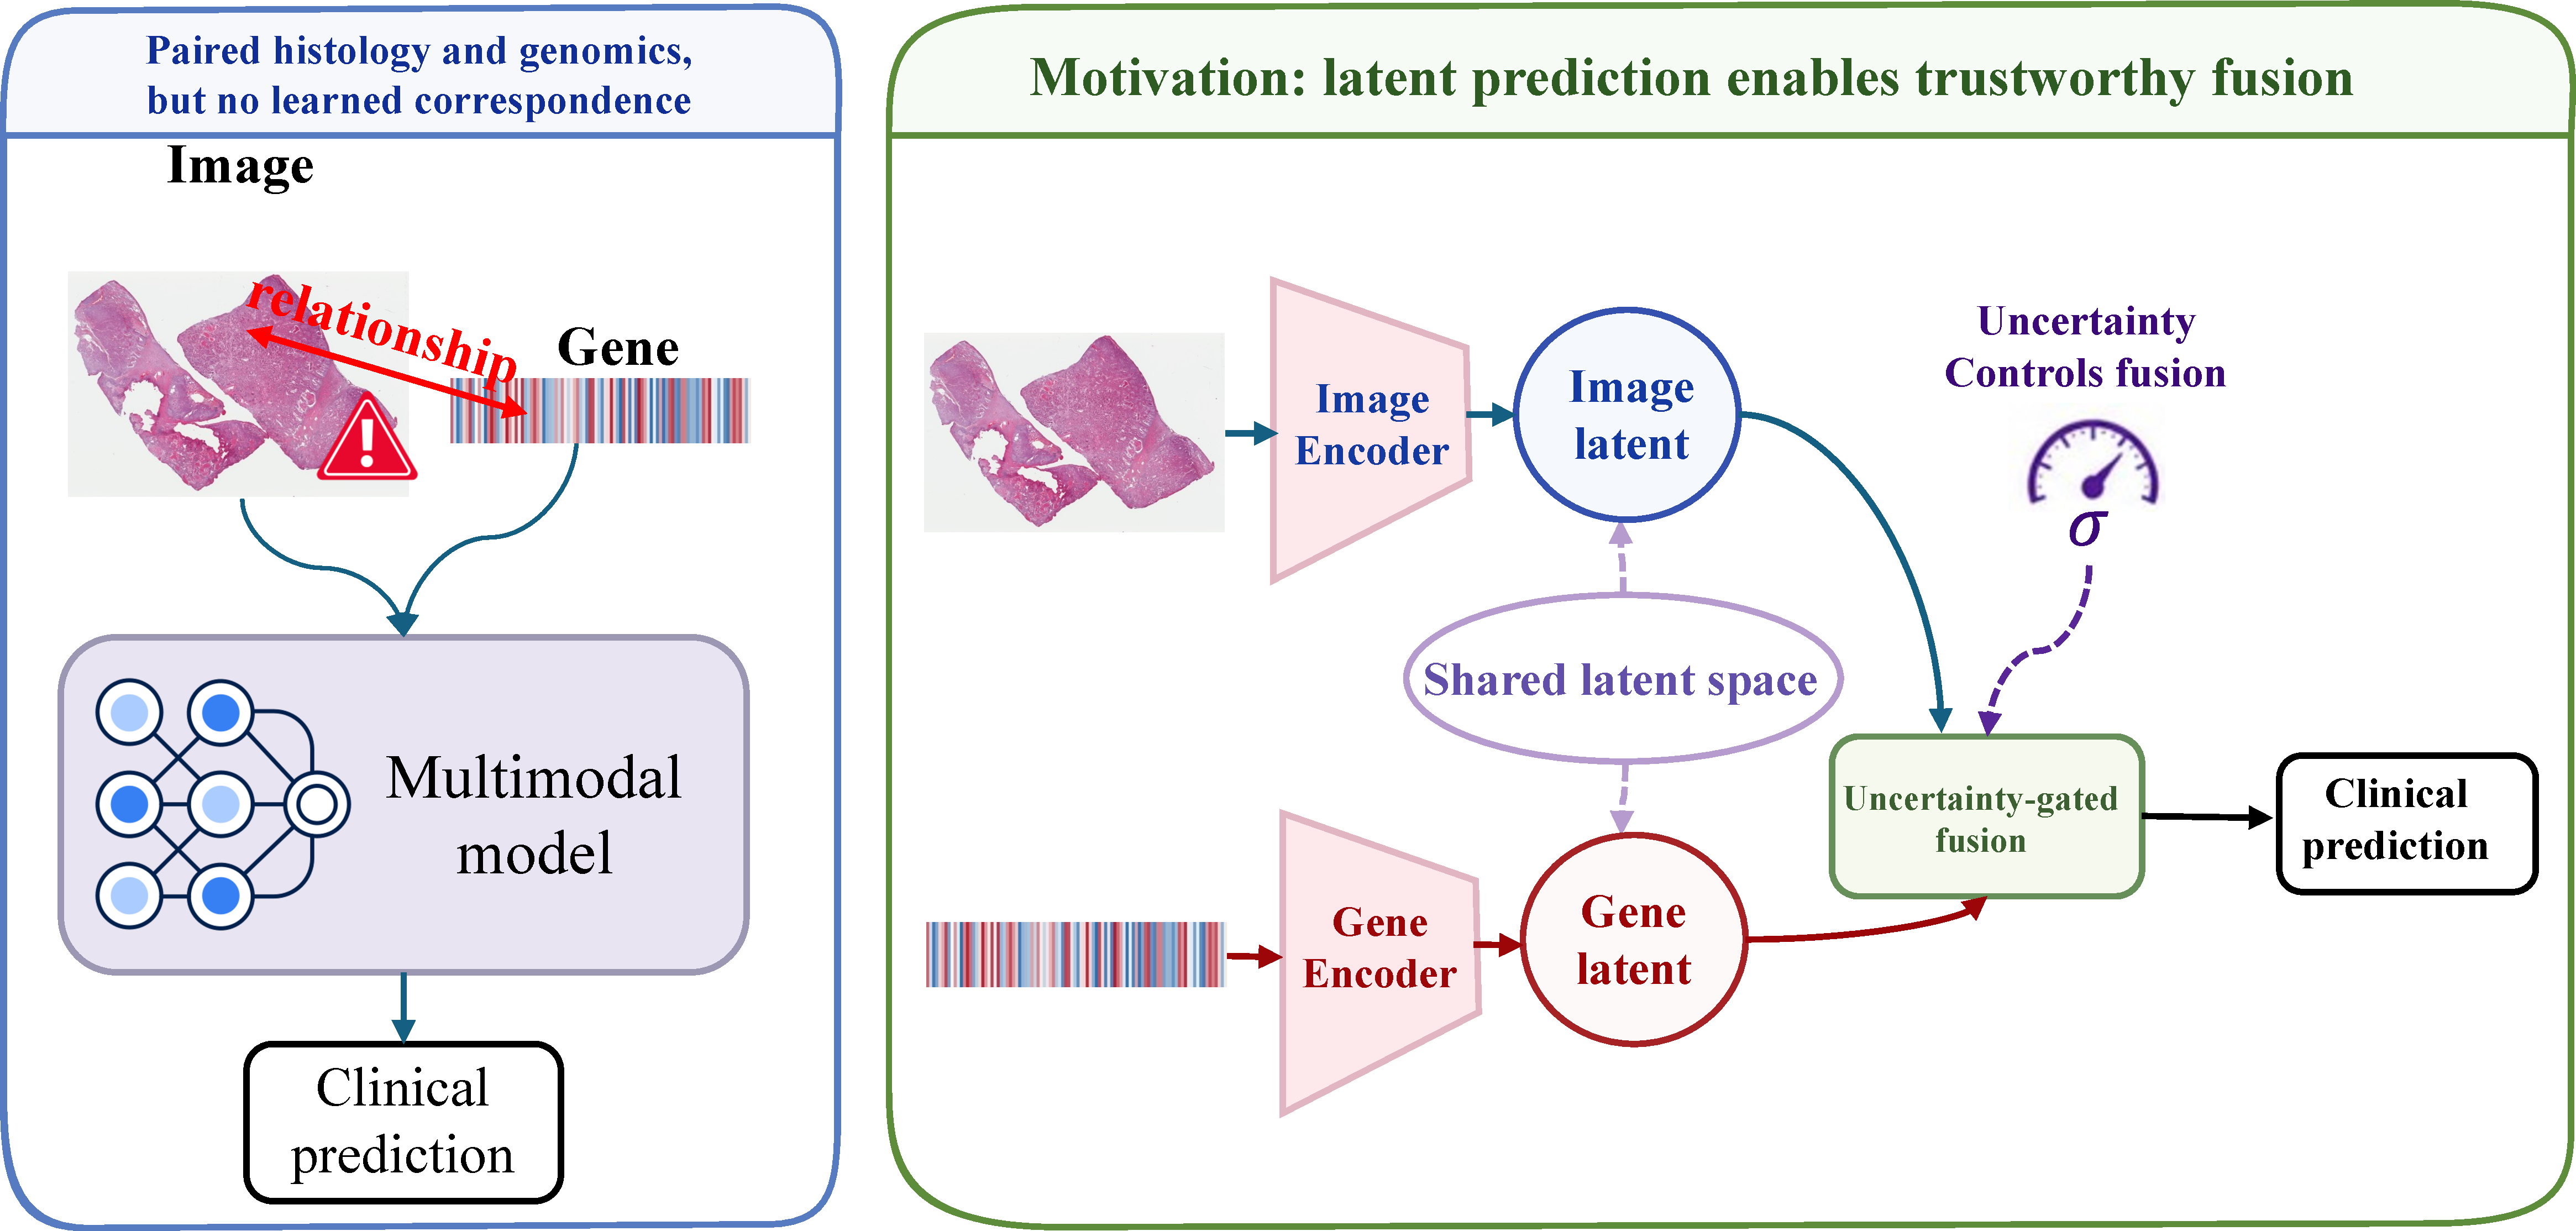
\includegraphics[width=0.8\linewidth]{figures/fig1.pdf}
    \caption{\textbf{Motivation.} JPathGene learns bidirectional latent prediction
and uncertainty-guided fusion.}
    \label{fig:overview}
\end{figure}


\section{Method}
\label{sec:method}

JPathGene comprises three stages (Fig.~2): modality-specific encoders
and EMA latent targets, bidirectional diffusion-JEPA for cross-modal
latent prediction, and CoRE-Fusion for uncertainty-guided residual
fusion. An optional InfoNCE objective aligns paired image and gene
latents. For each patient, $x_{\mathrm{img}}\in\mathbb{R}^{D}$ denotes
the pre-extracted histopathology feature vector, and
$x_{\mathrm{gene}}\in\mathbb{R}^{G}$ denotes the preprocessed genetic
feature vector.

\begin{figure}[t]
    \centering
    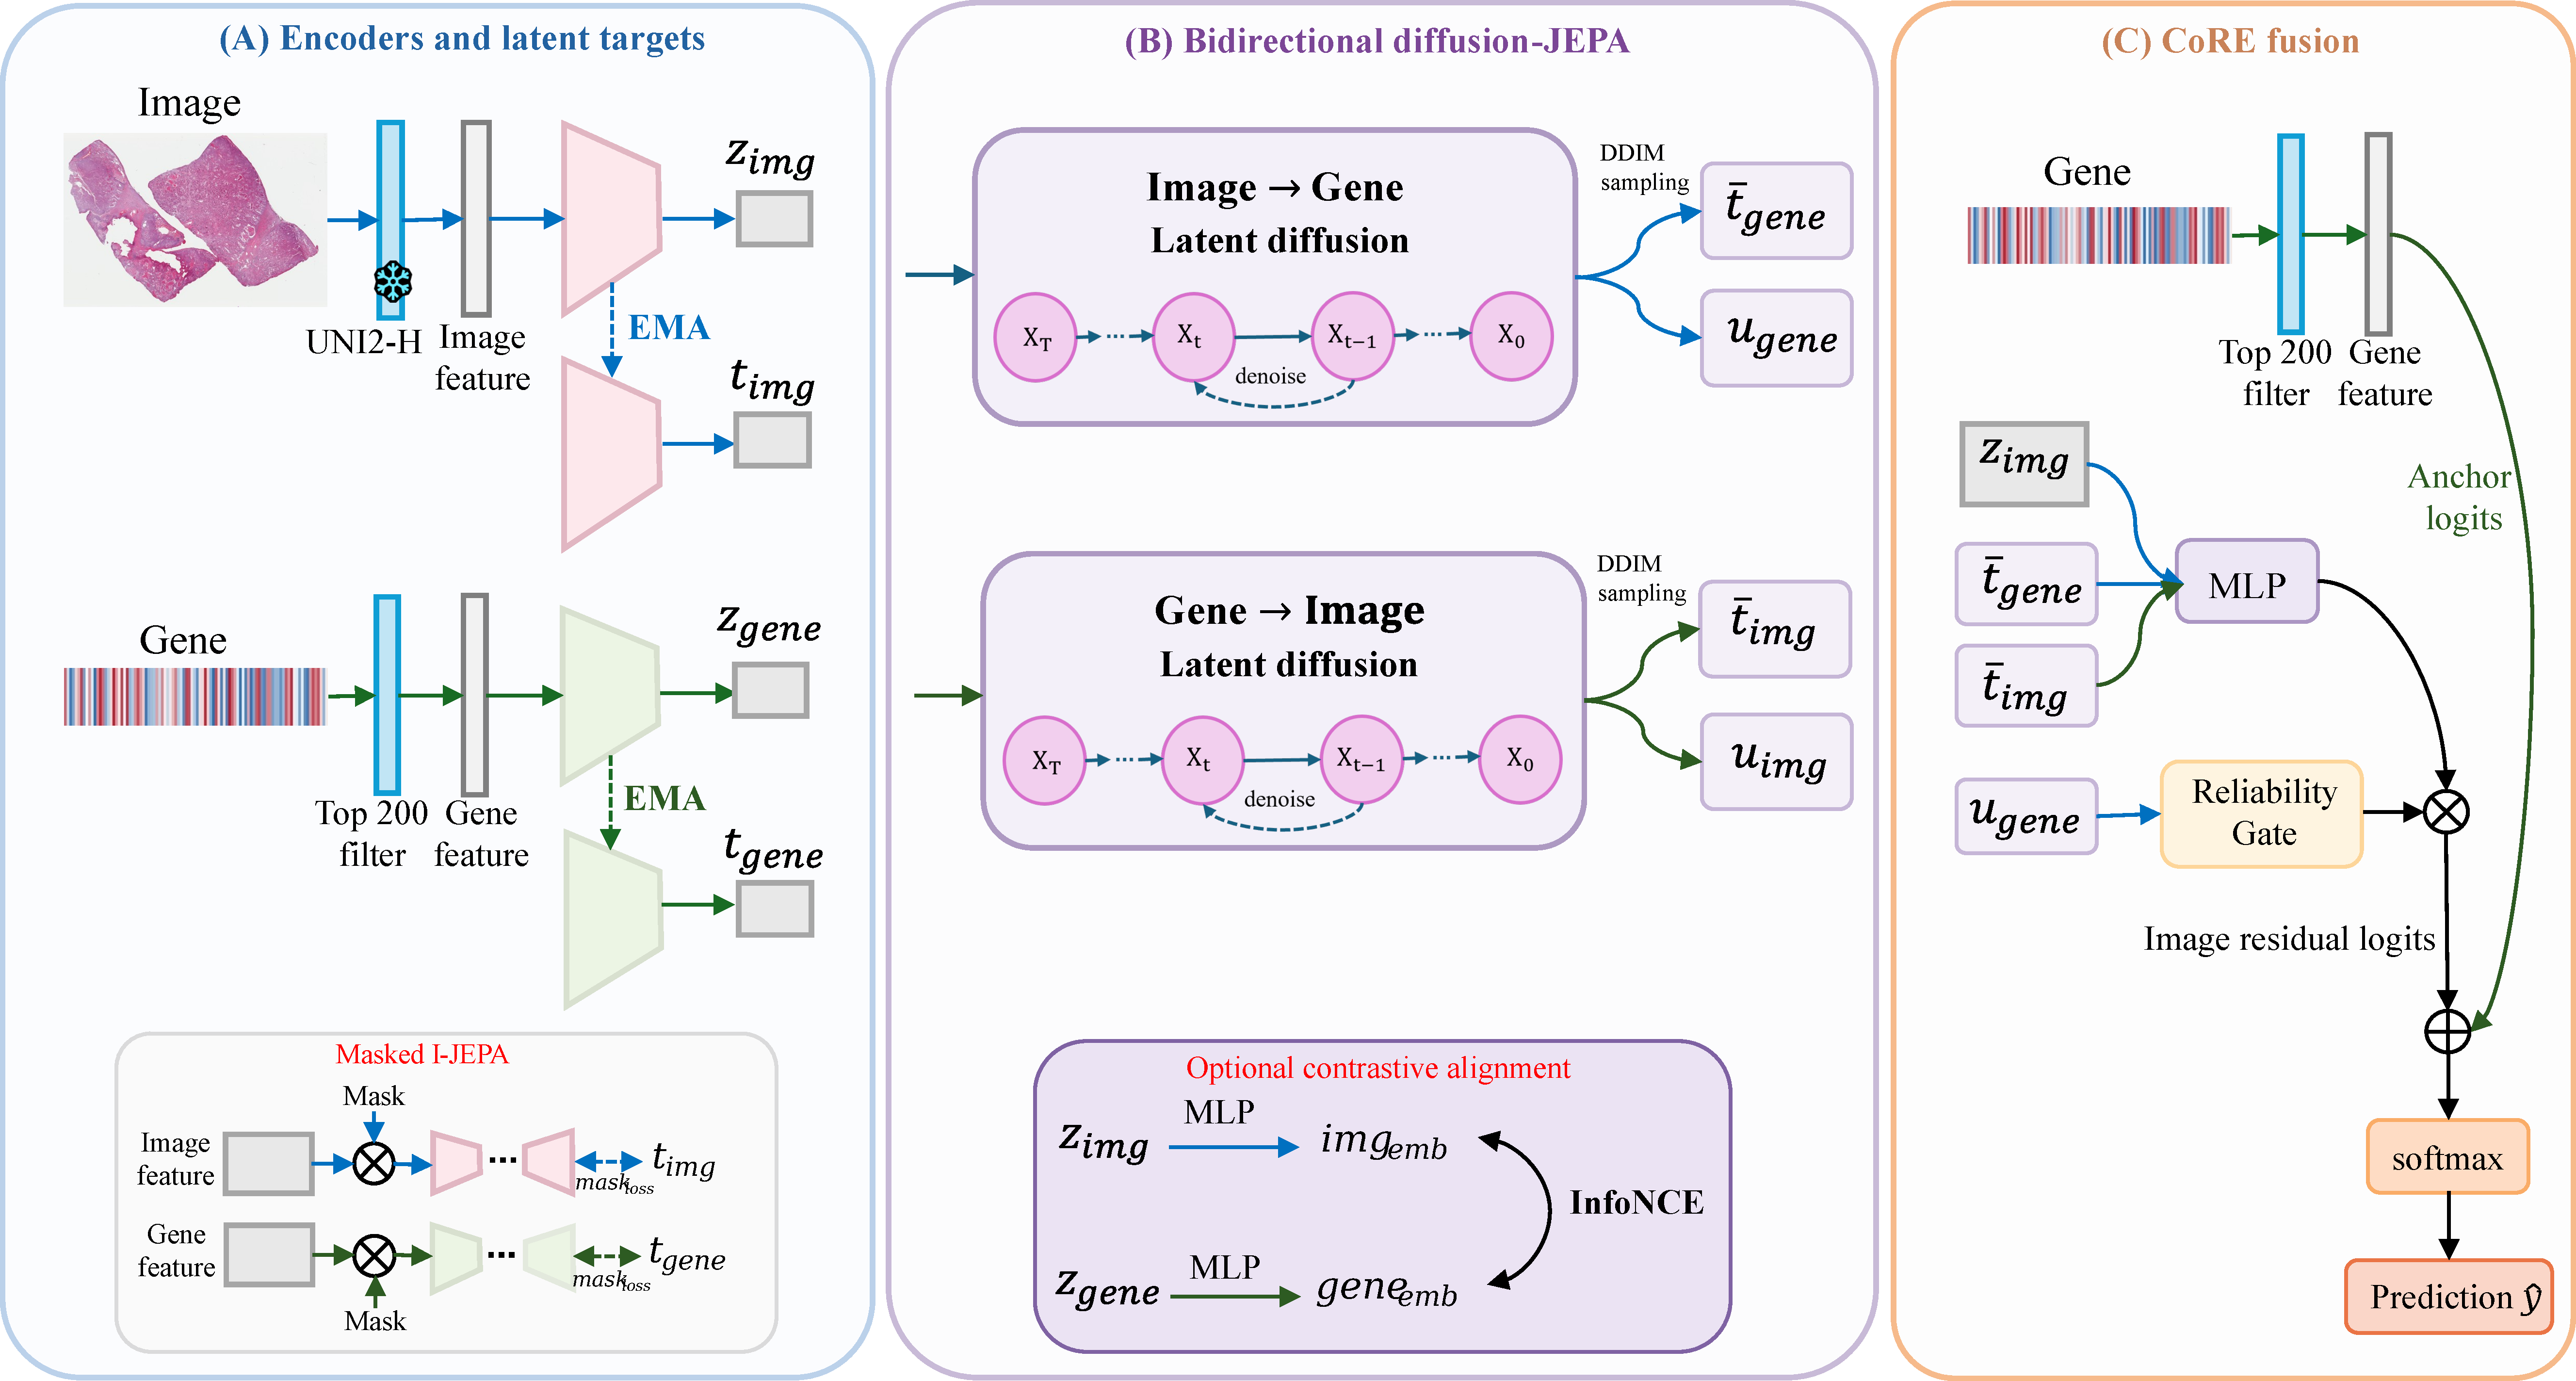
\includegraphics[width=0.95\linewidth]{figures/fig2.pdf}
    \caption{Overview of JPathGene.
(A) Online encoders and EMA teachers produce modality-specific latents and targets.
(B) Bidirectional diffusion-JEPA estimates cross-modal latent means and uncertainties.
(C) CoRE-Fusion uses uncertainty to gate an image residual over genomic anchor logits.}
    \label{fig:architecture}
\end{figure}

\subsection{Encoders and latent targets}
Figure~2A summarizes the online encoders, EMA teachers, and auxiliary masked I-JEPA objective. JPathGene uses pre-extracted histopathology features from a frozen UNI2-h encoder \cite{chen2024uni} and the highest-variance RNA-seq genes. Online encoders $f_{\mathrm{img}}$ and $f_{\mathrm{gene}}$ map them to shared $d$-dimensional latents $\mathbf{z}_{\mathrm{img}}$ and $\mathbf{z}_{\mathrm{gene}}$, using an MLP with optional attention-MIL pooling \cite{ilse2018attention} for images and an MLP or TabTransformer-style tokenizer \cite{huang2020tabtransformer,gorishniy2021ftt} for genes. EMA teachers, updated with momentum $m$, provide stop-gradient targets to prevent collapse. The gene target $t_{\mathrm{gene}}$ is an EMA latent, train-only PCA representation, or pathway-score vector \cite{subramanian2005gsea,liberzon2015hallmark}, while $t_{\mathrm{img}}$ is the image EMA latent. Thus, the model predicts compact latent targets rather than reconstructing raw gene-expression values.

\subsection{Cross-modal diffusion-JEPA}
\label{sec:diffusion}
Figure~2B summarizes bidirectional latent diffusion and DDIM sampling. Deterministic JEPA predicts a single target, but because one histologic phenotype can correspond to multiple genetic programs, we instead model $p(t_{\mathrm{gene}}\mid z_{img})$ and $p(t_{\mathrm{img}}\mid z_{gene})$ with a FiLM-conditioned \cite{perez2018film} latent-diffusion denoiser $\epsilon_\theta$ under a cosine noise schedule $\bar\alpha_\tau$ \cite{ho2020ddpm,nichol2021improved,song2021score}. Because the downstream classifier primarily uses posterior means,
diffusion is not expected to improve point prediction by itself.
Its main role is to represent a conditional latent distribution and
provide patient-specific uncertainty through repeated sampling.

Training follows the standard noise-prediction objective. At a random timestep
$\tau$, a target latent $t$ is perturbed as
$t^{(\tau)}=\sqrt{\bar\alpha_\tau}t+
\sqrt{1-\bar\alpha_\tau}\epsilon$, and $\epsilon_\theta$ predicts the added
noise $\epsilon$ conditioned on the source latent. The same predictor also supports the within-modality masked I-JEPA task \cite{assran2023ijepa}, where the context is a $\rho$-masked view, with deterministic JEPA as the single-step special case (Algorithm~\ref{alg:step}). During both training and inference, $N=8$ DDIM samples \cite{song2021ddim} conditioned on $\zimg$ estimate the posterior mean $\bar t_{\mathrm{gene}}$ and patient-specific uncertainty $u_{\mathrm{gene}}=\tfrac{1}{d}\sum_{j=1}^{d}\operatorname{std}_{n}[\hat t_{\mathrm{gene},j}^{n}]$; the uncertainty feeds the CoRE gate below, so sampling is part of each training step. Here, $t_{\mathrm{gene}}\in\mathbb{R}^{d}$ denotes the full genetic target latent, and $\hat t_{\mathrm{gene},j}^{n}$ denotes the $j$-th component of its $n$-th sampled prediction; $\bar t_{\mathrm{img}}$ and $u_{\mathrm{img}}$ are defined analogously.

\begin{algorithm}[t]
\caption{JPathGene training}
\label{alg:step}
\begin{algorithmic}[1]
\Require paired data $\mathcal{D}\!=\!\{(x^{\mathrm{img}}_i,x^{\mathrm{gene}}_i,y_i)\}$; online encoders $f_{\mathrm{img}},f_{\mathrm{gene}}$, denoiser $\epsilon_\theta$, projection heads $h_{\mathrm{img}},h_{\mathrm{gene}}$, fusion heads $g_{\mathrm{anchor}},g_{\mathrm{img}}$, gate $(w,b)$; EMA decay $m$; loss weights $\lambda_k$
\For{each training epoch}
\For{each minibatch $(x^{\mathrm{img}},x^{\mathrm{gene}},y)\in\mathcal{D}$}
\State $\zimg\!\gets\!f_{\mathrm{img}}(x^{\mathrm{img}})$, $\zgene\!\gets\!f_{\mathrm{gene}}(x^{\mathrm{gene}})$ \Comment{online (student) latents}
\State $t_{\mathrm{img}},t_{\mathrm{gene}}\!\gets\!\textsc{StopGrad}$ EMA teachers \Comment{or PCA/pathway $t_{\mathrm{gene}}$}
\State draw $\tau\!\sim\!\mathcal{U}\{1,T\}$, $\epsilon\!\sim\!\mathcal{N}(0,I)$; $\;t^{(\tau)}\!\gets\!\sqrt{\bar\alpha_\tau}\,t+\sqrt{1-\bar\alpha_\tau}\,\epsilon$
\State $\mathcal{L}_{\mathrm{i\to g}}\!\gets\!\|\epsilon-\epsilon_\theta(t^{(\tau)}_{\mathrm{gene}},\tau,\zimg)\|_2^2$; symmetric $\mathcal{L}_{\mathrm{g\to i}}$ \Comment{cross-modal JEPA}
\State $\mathcal{L}^{\mathrm{mask}}_{\mathrm{gene}}\!\gets\!\|\epsilon-\epsilon_\theta(t^{(\tau)}_{\mathrm{gene}},\tau,\zgene^{\mathrm{ctx}})\|_2^2$; symmetric $\mathcal{L}^{\mathrm{mask}}_{\mathrm{img}}$ \Comment{$\rho$-masked, same $\epsilon_\theta$}
\State $\mathcal{L}_{\mathrm{align}}\!\gets\!\textsc{InfoNCE}(h_{\mathrm{img}}(\zimg),h_{\mathrm{gene}}(\zgene))$ \Comment{optional}
\State $\bar t_{\mathrm{gene}},\bar t_{\mathrm{img}},u_{\mathrm{gene}}\!\gets\!\textsc{DDIM-Sample}(\epsilon_\theta,N)$ \Comment{mean + uncertainty, no grad}
\State $\alpha\!\gets\!\sigma\!\big(w(-u_{\mathrm{gene}})+b\big)$; $\;\hat y\!\gets\!g_{\mathrm{anchor}}(x^{\mathrm{gene}})+\alpha\,g_{\mathrm{img}}([\zimg,\bar t_{\mathrm{gene}},\bar t_{\mathrm{img}}])$; $\;\mathcal{L}_{\mathrm{cls}}\!\gets\!\mathrm{CE}(\hat y,y)$ \Comment{CoRE gate}
\State $\mathcal{L}\!\gets\!\textstyle\sum_{k}\lambda_k\mathcal{L}_k$, $k\in\{$i$\to$g, g$\to$i, mask, align, cls$\}$; update online $\Theta$ by $\nabla_\Theta\mathcal{L}$
\State EMA-update teachers: $\theta^{-}\!\gets\!m\,\theta^{-}+(1-m)\,\theta$
\EndFor
\EndFor
\end{algorithmic}
\end{algorithm}

\subsection{CoRE: complementary residual experts}
\label{sec:core}
For molecular endpoints, genomic features are often more predictive than histology, so naive multimodal fusion may underperform a gene-only model. \textbf{CoRE-Fusion} therefore retains a genomic anchor $g_{\mathrm{anchor}}(x_{\mathrm{gene}})$ and adds an uncertainty-gated image residual (Fig.~\ref{fig:architecture}):
\begin{equation}
\begin{aligned}
\hat{y}
&= g_{\mathrm{anchor}}(x_{\mathrm{gene}})
 + \alpha\, g_{\mathrm{img}}
 \bigl([z_{\mathrm{img}},\bar{t}_{\mathrm{gene}},
 \bar{t}_{\mathrm{img}}]\bigr), \\
\alpha
&= \sigma(-w u_{\mathrm{gene}}+b)\in(0,1).
\end{aligned}
\end{equation}
where $\sigma$ is the logistic function and $b$ and $w$ are learned scalars.
Both $g_{\mathrm{anchor}}$ and $g_{\mathrm{img}}$ output classification logits,
which are summed. The gate maps cross-modal uncertainty to a patient-specific
image-residual weight. The reported models use the soft gate, which continuously adjusts
rather than hard-thresholds the image contribution. The total
objective combines cross-modal prediction, masked prediction,
latent alignment, and classification losses, with
$\lambda_{i\rightarrow g}=\lambda_{g\rightarrow i}=\lambda_{\mathrm{cls}}=1$,
$\lambda_{\mathrm{mask}}=0.5$, and $\lambda_{\mathrm{align}}=0.1$,
and is optimized using AdamW.
\section{Experiments and Results}
\label{sec:experiments}

\subsection{Experimental setup}
Each cohort contains matched histopathology features, gene-expression features, and labels (Table~\ref{tab:datasets}). Our primary experiments use \textbf{TCGA-BRCA} \cite{weinstein2013tcga}, including 113 patients with both modalities. Histopathology is represented by slide-mean-pooled \textbf{UNI2-h} features \cite{chen2024uni}, and genomics by the 200 highest-variance RNA-seq genes. The TCGA-BRCA task predicts \textbf{estrogen-receptor (ER) status}, a molecular
binary endpoint with ER-negative as the positive class ($\approx21\%$), for which gene-only achieves an AUC of $0.95$. We further evaluate generalization on \textbf{TCGA-LUAD} using TP53 mutation prediction in 460 patients, with 48\% positives, and stage classification in 393 patients, distinguishing early stage from stage II or higher. Genomic features are highly predictive for TP53 mutation but less informative for stage. All splits are patient-level. Within each fold, normalization, top-variance
gene selection, PCA, and gene-target construction are fitted using training
patients only.

\begin{table}[t]
\centering
\caption{Paired TCGA cohorts using slide-mean-pooled UNI2-h features and the
200 highest-variance RNA-seq genes.}
\label{tab:datasets}
\resizebox{\linewidth}{!}{%
\begin{tabular}{llccccc}
\toprule
Cohort & Endpoint & Patients & Image dim & Gene dim & Classes & Pos.\ rate \\
\midrule
TCGA-BRCA (UNI2-h) & ER status & 113 & 1536 & 200 & 2 & 21\% \\
TCGA-LUAD (UNI2-h) & TP53 mut. & 460 & 1536 & 200 & 2 & 48\% \\
TCGA-LUAD (UNI2-h) & stage I vs II$+$ & 393 & 1536 & 200 & 2 & 44\% \\
\bottomrule
\end{tabular}%
}
\end{table}


The encoders produce $d{=}128$-dimensional latents. The diffusion predictor uses
FiLM conditioning and a cosine schedule ($T{=}1000$). Each forward pass draws
$N{=}8$ DDIM samples \cite{song2021ddim}, each with eight denoising steps per
direction, to estimate the posterior mean and uncertainty. EMA teachers use decay $0.996$ and
provide stop-gradient targets, and training uses AdamW on a single GPU. A
deterministic MLP attains a comparable AUC, indicating that diffusion is not
required for point prediction alone. Its role is instead to provide sample-based
patient uncertainty for CoRE and to represent the one-to-many
histology-to-genomics mapping.

\paragraph{Baselines and evaluation.}
We compare image-only and gene-only models with early, late, concatenation,
gated, and cross-attention fusion, contrastive alignment, and TabTransformer
\cite{huang2020tabtransformer}, using identical encoders and training settings.
We report AUC, F1, ECE, Brier score, and NLL. Results are mean$\pm$std over five
seeds, with Welch $t$-tests on per-seed values. ECE uses 15-bin top-label
calibration \cite{guo2017calibration} on pooled out-of-fold predictions without
post-hoc scaling; because ECE is binning-sensitive on the small BRCA cohort, we
treat the binning-free Brier score and NLL as the primary calibration evidence.

\subsection{TCGA-BRCA results and ablation}
\label{sec:uni}
Among fourteen evaluated methods (Table~\ref{tab:uni_compare}), JPathGene
achieves the highest multimodal AUC and matches gene-only
($0.954$ vs.\ $0.954$; n.s.), while substantially reducing ECE relative to
gene-only ($0.094$ vs.\ $0.229$, $p\!<\!0.001$). This benefit is feature-dependent: with generic $2048$-dimensional ResNet-50
features the ordering reverses -- simple early and gated fusion lead (AUC $0.94$)
while JPathGene and gene-only trail ($\approx\!0.91$) -- and only with UNI2-h does
cross-modal learning reach the top. On pooled BRCA out-of-fold predictions,
JPathGene changes $26\%$ of gene-only decisions at the $0.5$ threshold and shifts
predicted probabilities by more than $0.10$ for $82\%$ of patients. Full has
lower F1 because its conservative probabilities reduce recall at the fixed
$0.5$ threshold, whereas CoRE recovers F1 through the gene anchor at the cost
of higher ECE. The variants therefore trade calibration against thresholded
classification performance.

\begin{table}[t]
\centering
\caption{TCGA-BRCA comparison using UNI2-h features and leakage-safe
5-fold$\times$5-seed CV (mean$\pm$std). Best AUC and ECE are bold.}
\label{tab:uni_compare}
\begin{tabular}{lccc}
\toprule
Method & AUC\,$\uparrow$ & F1\,$\uparrow$ & ECE\,$\downarrow$ \\
\midrule
\multicolumn{4}{l}{\emph{Unimodal}}\\
Gene-only & \textbf{0.954\,$\pm$\,0.018} & 0.748\,$\pm$\,0.066 & 0.229\,$\pm$\,0.024 \\
Image-only & 0.775\,$\pm$\,0.025 & 0.367\,$\pm$\,0.210 & 0.104\,$\pm$\,0.010 \\
\midrule
\multicolumn{4}{l}{\emph{Multimodal fusion baselines}}\\
Concat fusion & 0.928\,$\pm$\,0.033 & 0.392\,$\pm$\,0.127 & 0.088\,$\pm$\,0.027 \\
Contrastive (CLIP-style) & 0.927\,$\pm$\,0.052 & 0.436\,$\pm$\,0.203 & 0.081\,$\pm$\,0.023 \\
Late fusion & 0.917\,$\pm$\,0.037 & 0.534\,$\pm$\,0.165 & 0.079\,$\pm$\,0.022 \\
Early fusion & 0.915\,$\pm$\,0.044 & 0.683\,$\pm$\,0.080 & 0.099\,$\pm$\,0.029 \\
Cross-attention & 0.910\,$\pm$\,0.037 & 0.470\,$\pm$\,0.109 & 0.078\,$\pm$\,0.014 \\
Gated fusion & 0.890\,$\pm$\,0.042 & 0.515\,$\pm$\,0.093 & 0.087\,$\pm$\,0.017 \\
TabTransformer concat & 0.807\,$\pm$\,0.024 & 0.497\,$\pm$\,0.062 & 0.119\,$\pm$\,0.027 \\
\midrule
\multicolumn{4}{l}{\emph{JPathGene (ours)}}\\
\textbf{Full} & \textbf{0.954\,$\pm$\,0.010} & 0.602\,$\pm$\,0.122 & 0.094\,$\pm$\,0.033 \\
\textbf{CoRE} & 0.953\,$\pm$\,0.016 & 0.743\,$\pm$\,0.034 & 0.190\,$\pm$\,0.039 \\
\textbf{MLP predictor} & 0.941\,$\pm$\,0.022 & 0.466\,$\pm$\,0.125 & 0.080\,$\pm$\,0.021 \\
\textbf{Diffusion (PCA)} & 0.916\,$\pm$\,0.046 & 0.593\,$\pm$\,0.132 & \textbf{0.071\,$\pm$\,0.020} \\
\textbf{Full (diff.+pathway)} & 0.882\,$\pm$\,0.041 & 0.495\,$\pm$\,0.110 & 0.076\,$\pm$\,0.013 \\
\bottomrule
\end{tabular}
\end{table}

\paragraph{Calibration.}
\label{sec:calib}
Because ECE is binning-sensitive, we additionally report Brier score and NLL
(Table~\ref{tab:calibration}). JPathGene attains the lowest Brier score ($0.089$)
and NLL ($0.276$), compared with $0.147$ and $0.463$ for gene-only, indicating
better probabilistic predictions beyond bin-based calibration.

\begin{table}[t]
\centering
\caption{Proper scoring rules on pooled out-of-fold predictions
(mean$\pm$std over five seeds; lower is better). Best values are bold.}
\label{tab:calibration}
\begin{tabular}{lcc}
\toprule
Method & Brier & NLL \\
\midrule
Image-only & 0.140\,$\pm$\,0.007 & 0.495\,$\pm$\,0.029 \\
Gene-only & 0.147\,$\pm$\,0.059 & 0.463\,$\pm$\,0.141 \\
Concat fusion & 0.102\,$\pm$\,0.014 & 0.322\,$\pm$\,0.041 \\
\textbf{JPathGene (ours)} & \textbf{0.089\,$\pm$\,0.014} & \textbf{0.276\,$\pm$\,0.033} \\
\bottomrule
\end{tabular}
\end{table}

\paragraph{Ablation.}
A $2^4$ factorial ablation identifies the gene anchor as the dominant component,
with anchored configurations reaching AUC $0.94$--$0.96$ versus
$0.84$--$0.92$ without it. Masked and cross-modal JEPA reduce variance,
whereas contrastive alignment adds little benefit.

\subsection{TCGA-LUAD validation}
\label{sec:luad}
We further evaluate JPathGene on TCGA-LUAD
(Table~\ref{tab:luad_combined}). For TP53 mutation, CoRE significantly
outperforms gene-only in both AUC ($0.793$ vs.\ $0.774$, $p\!=\!0.028$)
and calibration ($p\!=\!0.041$). For stage classification, all multimodal
methods improve AUC by $0.07$--$0.11$ over gene-only ($p\!<\!0.001$),
indicating complementary histologic information. The gate therefore adjusts
the image contribution according to cross-modal reliability.
Figure~\ref{fig:qualitative} shows held-out cases recovered by JPathGene when
the unimodal and concatenation models fail.

\begin{table}[t]
\centering
\caption{TCGA-LUAD validation using UNI2-h features and
5-fold$\times$5-seed CV (mean$\pm$std).
Best AUC and ECE per endpoint are bold.}
\label{tab:luad_combined}
\resizebox{\linewidth}{!}{%
\begin{tabular}{lcccc}
\toprule
& \multicolumn{2}{c}{TP53 mutation ($n{=}460$)} & \multicolumn{2}{c}{Stage early/II$+$ ($n{=}393$)} \\
\cmidrule(lr){2-3}\cmidrule(lr){4-5}
Method & AUC & ECE & AUC & ECE \\
\midrule
Image-only & 0.693\,$\pm$\,0.013 & 0.237\,$\pm$\,0.044 & 0.662\,$\pm$\,0.032 & 0.224\,$\pm$\,0.023 \\
Gene-only & 0.774\,$\pm$\,0.006 & 0.181\,$\pm$\,0.041 & 0.578\,$\pm$\,0.014 & \textbf{0.166\,$\pm$\,0.031} \\
Concat fusion & 0.764\,$\pm$\,0.012 & 0.202\,$\pm$\,0.042 & 0.650\,$\pm$\,0.017 & 0.230\,$\pm$\,0.029 \\
Late fusion & 0.745\,$\pm$\,0.013 & 0.209\,$\pm$\,0.027 & \textbf{0.684\,$\pm$\,0.019} & 0.209\,$\pm$\,0.033 \\
\textbf{JPathGene (full, ours)} & 0.769\,$\pm$\,0.019 & 0.195\,$\pm$\,0.025 & 0.661\,$\pm$\,0.013 & 0.227\,$\pm$\,0.042 \\
\textbf{JPathGene (gene-anchored, ours)} & 0.770\,$\pm$\,0.017 & 0.183\,$\pm$\,0.041 & 0.669\,$\pm$\,0.012 & 0.188\,$\pm$\,0.039 \\
\textbf{JPathGene (CoRE, ours)} & \textbf{0.793\,$\pm$\,0.012} & \textbf{0.118\,$\pm$\,0.028} & 0.669\,$\pm$\,0.011 & 0.223\,$\pm$\,0.026 \\
\bottomrule
\end{tabular}%
}
\end{table}


\begin{figure}[!htb]
    \centering
    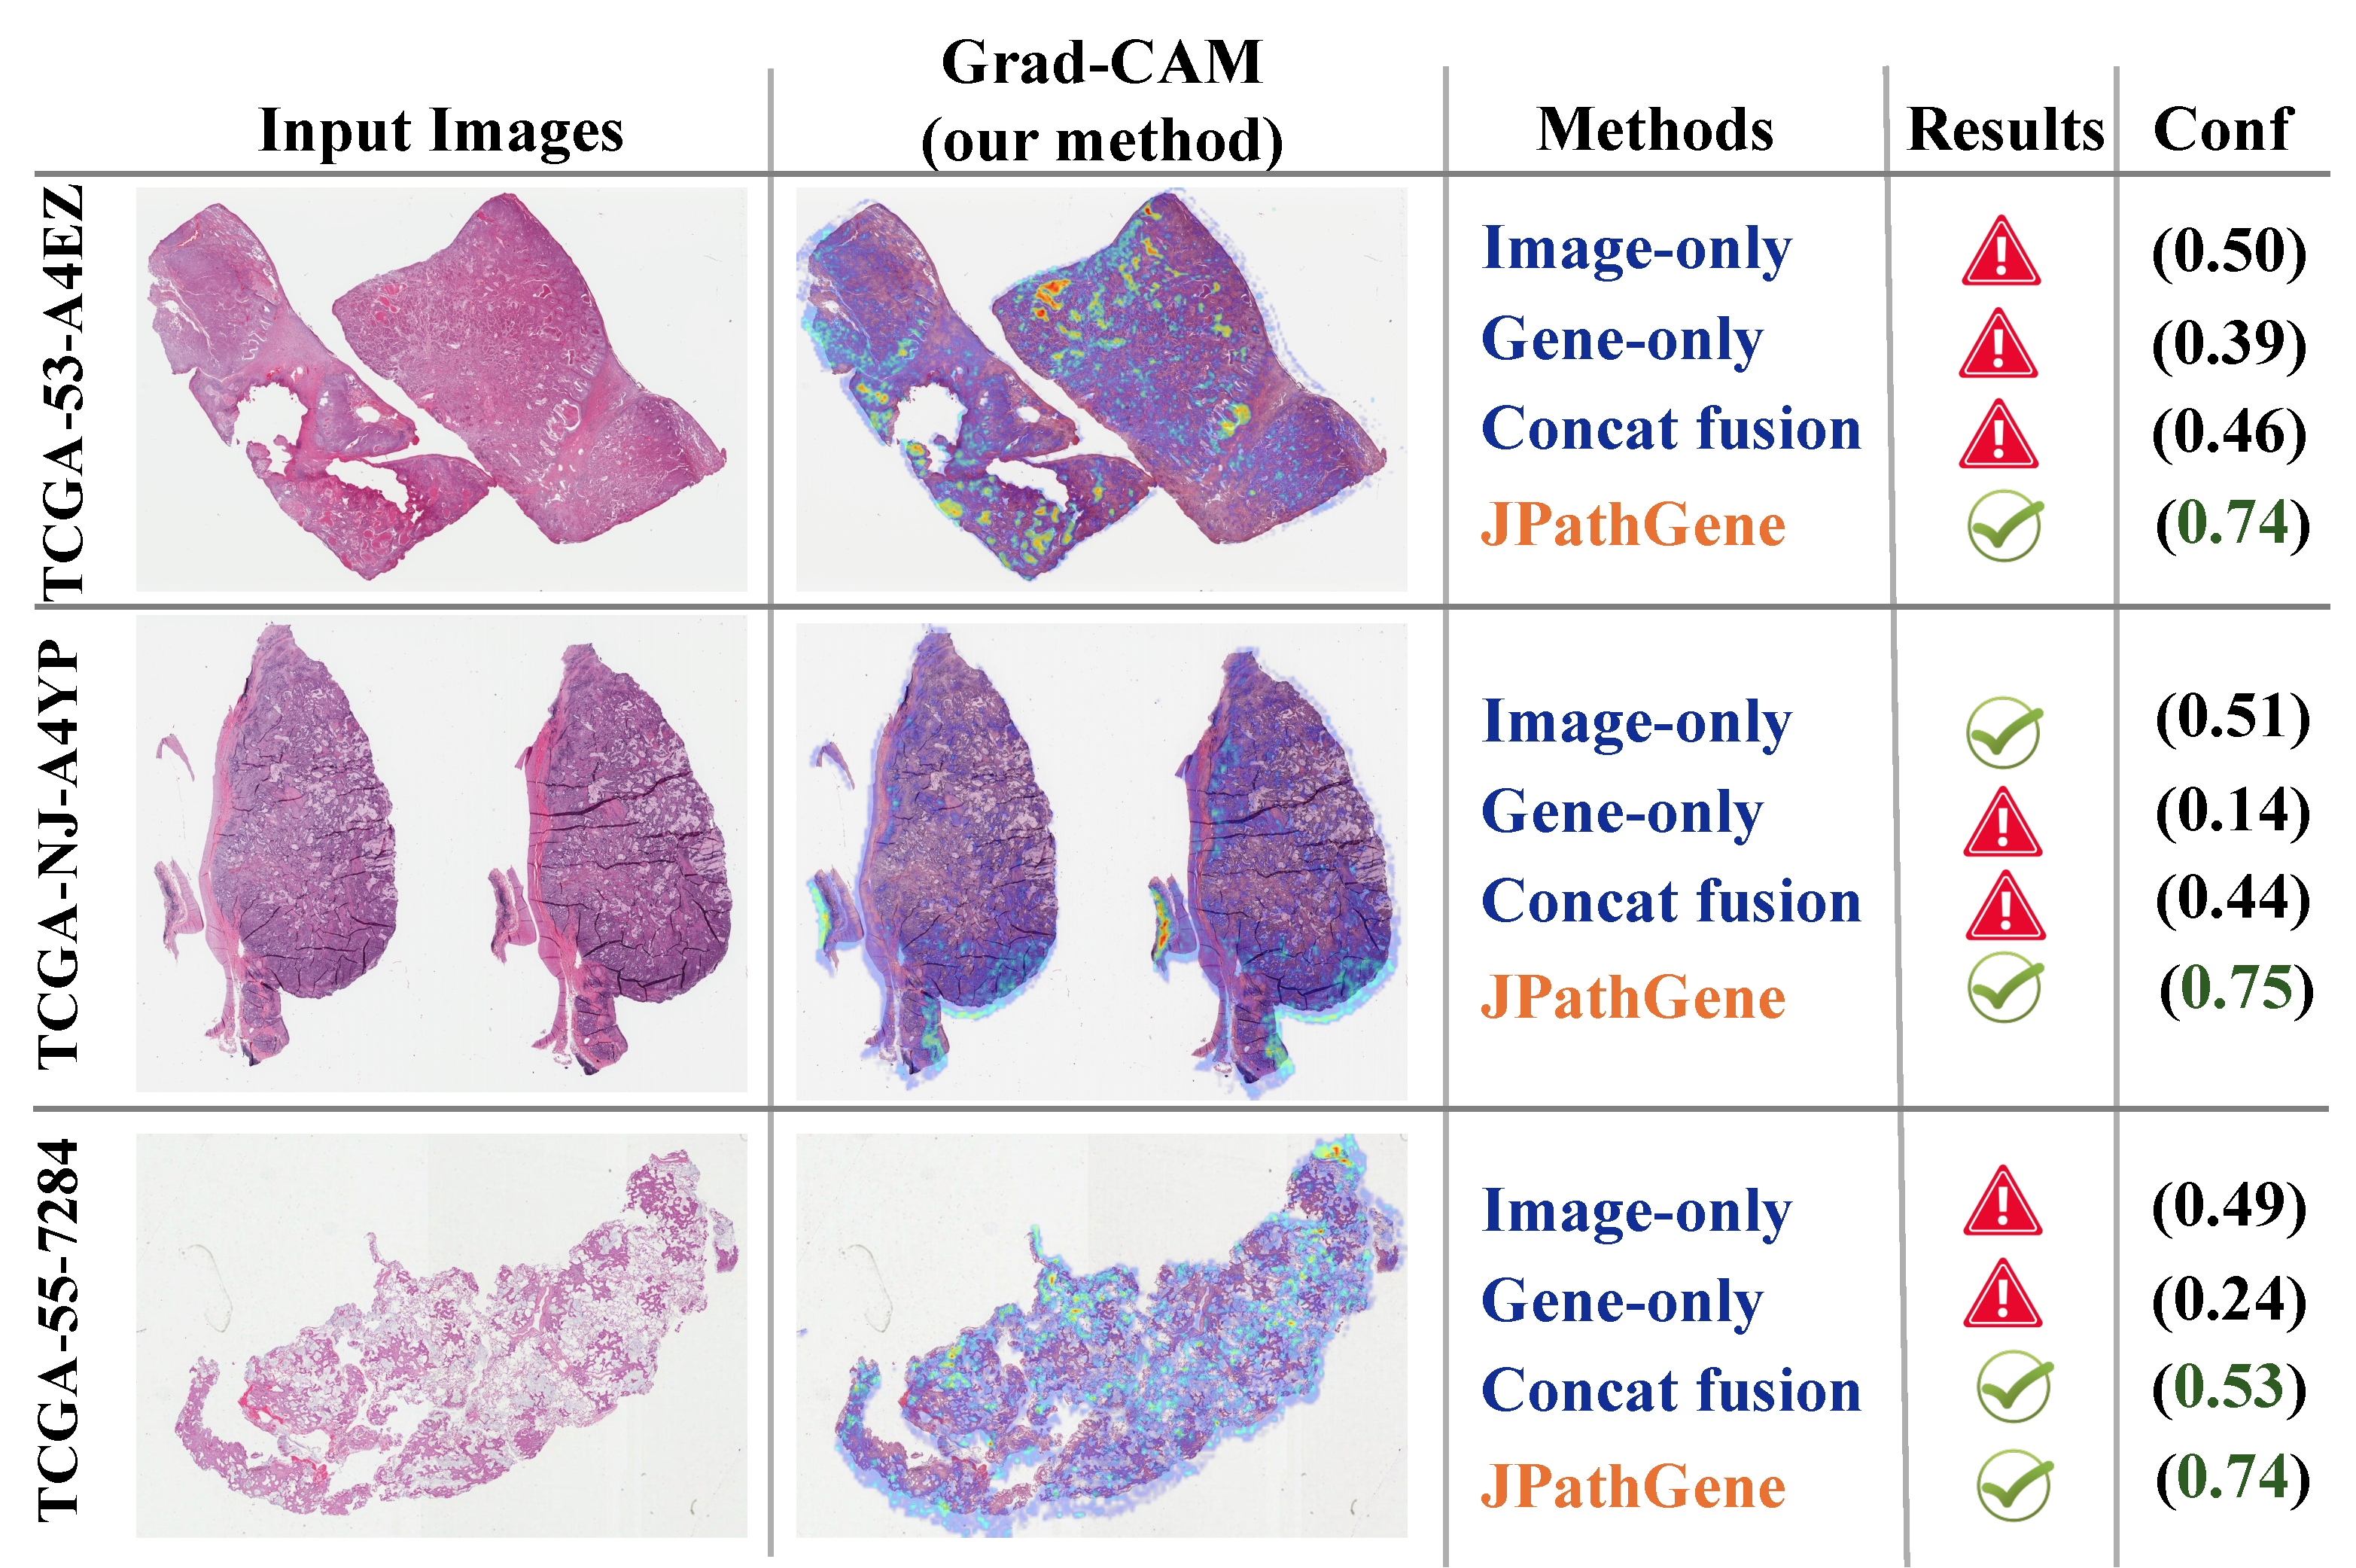
\includegraphics[width=0.8\linewidth]{figures/fig3.pdf}
    \caption{\textbf{LUAD-stage examples.} JPathGene correctly classifies
held-out cases missed by image-only, gene-only, and concatenation fusion.}
    \label{fig:qualitative}
\end{figure}

\FloatBarrier
\section{Conclusion}
\label{sec:conclusion}

JPathGene formulates histopathology--genomics fusion as bidirectional latent
diffusion prediction and uses sample-based uncertainty to gate an image residual
over a genomic anchor. Its benefit depends on feature quality and endpoint type,
matching gene-only on TCGA-BRCA, outperforming it on LUAD-TP53, and improving
LUAD-stage AUC by $0.08$--$0.09$. Unlike evidential or Dempster--Shafer fusion
\cite{sensoy2018evidential,han2021trusted}, CoRE uses cross-modal sampling
variance to adapt the per-patient image-residual weight. Current limitations include pre-extracted features, approximate gene
targets, additional sampling, and the need for clinical validation. Future work
will study larger pan-cancer cohorts and spatially resolved molecular targets.


\FloatBarrier

\begin{credits}
\subsubsection{\discintname}
The authors have no competing interests to declare that are relevant to the content
of this article.
\end{credits}

\bibliographystyle{splncs04}
\bibliography{references}

\end{document}
